\subsection{30.11.18}
\subsubsection{Испытание Бернулли}
Пусть на произвольном вероятностном пространстве $(S, Pr)$ объявлена ДСВ $\xi$ такая, что $Pr\{\xi = 1\} = p, Pr\{\xi = 0\} = 1 - p$. Словами это можно обосновать так: каждый элементарный исход $\omega \in S$ считается либо успешным ($\xi(\omega) = 1$), либо неудачным ($\xi(\omega) = 0$). Тогда:\\
$E \xi = 0 * (1 - p) + 1 * p = p$\\
$D \xi = E \xi^2 - (E \xi)^2 = (1 - p) * 0^2 + p * 1^2 - p^2 = p - p^2 = p(1 - p)$
\subsubsection{Моделирование ДСВ, генераторы случайных чисел}
Многократно повторяемый эксперимент, исходы которого имеют заданный набор вероятностей, соответствующий набору вероятностей ДСВ, называют моделью этой ДСВ.\\
Пример: моделью $\xi$ ($Pr\{\xi = 0\} = \frac{1}{2}, Pr\{\xi = 1\} = \frac{1}{2}$) можно считать бросок монетки (если считать, что стороны монетки одинаковые, монетка никогда не падает на ребро и бросают ее наугад).\\
Многократно повторяемый эксперимент, результатом которого является (псевдо)случайно выбранное число из некоторого конечного множества, называют дискретным генератором (датчиком) случайных чисел.\\
Пример: назовем $\alpha$ дискретный генератор случайных чисел, для которого $Pr\{\alpha = k\} = \frac{1}{N} \; \forall k \in 1:N$.\\
Многократно повторяемый эксперимент, результатом которого является (псевдо)случайно выбранное число из некоторого промежутка числовой прямой, называют непрерывным генератором (датчиком) случайных чисел.\\
Пример: назовем $\alpha_0$ непрерывный генератор случайных чисел, который с равной вероятностью попадает в каждую из точек отрезка $[0, 1]$.\\
Поскольку отрезок $[0, 1]$ содержит несчетное количество точек, вероятность $Pr\{\alpha_0 = x\} = \frac{1}{\infty} = 0 \; \forall x \in [0, 1]$. Однако, вероятность того, что точка попадет в некоторый промежуток, все же ненулевая:\\
$Pr\{x \in <a, b>\} = \frac{|<a, a + \delta>|}{|[0, 1]|} = \frac{\delta}{1} = \delta$\\
В частности, $Pr\{x \in [0, 1]\} = 1$.\\
Замечание: поскольку для конкретной точки вероятность попадания туда $\alpha_0$ равна нулю, можно смело выкидывать из множества конечное (и даже счетное) количество точек, и вероятность попадания в него останется неизменной. Следовательно, вместо $<a, b>$ можно рассматривать $(a, b)$ или $[a, b)$. Последнее особенно удобно, поскольку полуинтервалы хорошо стыкуются.
\subsubsection{Табличный метод моделирования ДСВ}
Итак, пусть есть вероятностное пространство $(S, Pr)$ и заданная на нем ДСВ $\xi$.\\
При этом $S = \{0, 1, \; ... \; , n - 1\}$, $\forall i \in 0:(n - 1) \; Pr(\{i\}) = p_i$, $\sum\limits_{i = 0}^{n - 1} p_i = 1$.\\
Примечание: для ДСВ с произвольным набором значений можно их пронумеровать и свести задачу к данной.
Возьмем отрезок $[0, 1)$ и поделим его на полуинтервалы вида $[x_i, x_{i + 1})$, где $x_0 = 0$, $\forall i \in 0:(n - 1) \; x_{i + 1} = x_i + p_i$\\
Для такого разбиения отрезка $[0, 1]$ вероятность $Pr\{\alpha_0 \in [x_i, x_{i + 1}]\} = p_i$. То есть, эксперимент "в отрезок с каким номером попадет случайное число, выданное $\alpha_0$?" моделирует $\xi$.\\
Замечание: При попадании в точку 1 значение $\alpha_0$ оказывается вне пределов всех полуинтервалов. Но с одной стороны, вероятность такого события - 0, так что распределение вероятностей это нам не портит, а с другой, если это все же произошло, мы можем просто объявить эксперимент неудачным и провести его заново.\\
Основным недостатком данного метода является большое количество сравнений вещественных чисел, каковая операция является не очень точной и достаточно долгой. Неплохо бы придумать метод, который минимизирует количество таких операций.
\subsubsection{Метод Уокера}
В табличном методе мы располагали полуинтервалы на отрезке $[0, 1]$ в произвольном порядке. В этот раз мы сначала разделим его на полуинтервалы $[\frac{i}{n}, \frac{i + 1}{n}) \; \forall i \in 0:(n - 1)$ (назовем их базовыми полуинтервалами. Такого обозначения на лекции не было, но я не хочу каждый раз уточнять, имею я в виду эти полуинтервалы или те, длины которых равны вероятностям) и будем следить, чтобы в одном таком полуинтервале было не более одной границы полуинтервалов, соответствующих исходам. Более того, если раньше каждому исходу соответствовал ровно один полуинтервал, то сейчас их может быть несколько, главное только, чтобы сумма их длин все еще была равна вероятности этого исхода.\\
Зачем? Давайте посмотрим на число $n * \alpha_0$. \\
Утверждение: его целая часть $\lfloor n * \alpha_0 \rfloor$ будет равно i, если $\frac{i}{n} \leq \alpha_0 < \frac{i + 1}{n}$.\\
Доказательство: умножим все части неравенства на n: $i \leq n * \alpha_0 < i + 1 \Leftrightarrow \lfloor n * \alpha_0 \rfloor = i$.\\
Итак, мы научились понимать, в какой базовый полуинтервал попал $\alpha_0$. Теперь осталось понять, что делать, если в базовом полуинтервале есть граница между полуинтервалами. Пусть эта граница есть в точке $x, \frac{i}{n} \leq x < \frac{i + 1}{n}$. Растянем наш базовый полуинтервал в n раз:\\
Точка $\frac{i}{n}$ перейдет в точку $i = \lfloor n * \alpha_0 \rfloor$, $\alpha_0$ - в $n * \alpha_0$, x - в $n * x$, $\frac{i + 1}{n}$ - в $i + 1 = \lfloor n * \alpha_0 \rfloor + 1$.\\
Теперь сдвинем полуинтервал влево на i: $\lfloor n * \alpha_0 \rfloor$ перейдет в 0, $n * \alpha_0$ - в $\{n * \alpha_0\}$ (дробная часть), $n * x$ - в $n * x - i$, $\lfloor n * \alpha_0 \rfloor + 1$ - в 1. То есть, теперь нам достаточно сравнить $\{n * \alpha_0\}$ и $n * x - i$, причем $n * x - i$ не зависит от $\alpha_0$ и может быть посчитана заранее.\\
Замечание: при попадании в единицу нам все еще придется повторять опыт.\\
Итак, пусть каждому значению случайной величины $i \in 0:(n - 1)$ соответствует множество $P_i$ полуинтервалов, причем каждый из них полностью лежит в одном из базовых полуинтервалов и пересечение $P_i$ и $P_j$ пусто для любого $j \not= i$, а $\sum\limits_{[a, b) \in P_i}|[a, b)| = p_i$. Также, в каждом базовом полуинтервале лежит не более двух полуинтервалов.\\
Тогда мы научились с помощью двух сравнений понимать, в какой полуинтервал $[a, b)$ попал $\alpha_0$, а если объявить исходом эксперимента i, где $[a, b) \in P_i$, то этот эксперимент будет моделировать $\xi$, так как вероятность попасть в полуинтервал, лежащий в $P_i$ равна $\sum\limits_{[a, b) \in P_i}Pr\{\alpha_0 \in [a, b)\} = \sum\limits_{[a, b) \in P_i}|[a, b)| = p_i$ Осталось только построить такое разбиение.\\
Для этого нам придется доказать две леммы:\\
Лемма 1: если $n > 1$, $\exists l \in 0:(n - 1): \; p_l \leq \frac{1}{n}$. Доказательство: если нет, то $\sum\limits_{i = 0}^{n - 1} p_i > 1$.\\
Лемма 2: если $n > 1$, $\forall l \in 0:(n - 1) \; \exists m \in 0:(n - 1), m \not= l : \; p_l + p_m > \frac{1}{n}$. Доказательство: если нет, то $\exists l_0 \in 0:(n - 1)$ такое, что:\\
$\sum\limits_{m \not= l_0} (p_{l_0} + p_m) \leq \frac{n - 1}{n} < 1$\\
С другой стороны, $\sum\limits_{m \not= l_0} (p_{l_0} + p_m) = \sum\limits_{m \not= l_0} p_{l_0} + \sum\limits_{m \not= l_0}p_m = (n - 1) * p_{l_0} + \sum\limits_{m \in 0:(n - 1)}p_m \geq 1$. Противоречие.\\
Итак, начнем строить наше разбиение:\\
Определим $\xi^{(0)}: p^{(0)}_i = p_i$, выберем $l_0: \; p^{(0)}_{l_0} < \frac{1}{n}$, $m_0: \; p^{(0)}_{l_0} + p^{(0)}_{m_0} > \frac{1}{n}$\\
Определим ДСВ $\psi^{(0)}: \; Pr\{\psi^{(0)} = l_0\} = n * p^{(0)}_{l_0}\}, Pr\{\psi^{(0)} = m_0\} = 1 - n * p^{(0)}_{l_0}\}$.\\
Теперь отрежем от отрезка $[0, 1]$ первый базовый полуинтервал:\\
$\xi^{(1)}: p^{(1)}_{l_0} = 0, p^{(1)}_{m_0} = (p^{(0)}_{m_0} - (\frac{1}{n} - p^{(0)}_{l_0})) * \frac{n}{n - 1},  p^{(1)}_i = p_i * \frac{n}{n - 1}$ и перейдем к следующему шагу алгоритма.\\
Теперь научимся вычислять $\forall k \in 0:(n - 1) \; p^{(0)}_i$ через $\xi^{(1)}$:\\
$p^{(0)}_k = \frac{1}{n}Pr\{\psi^{(0)} = k\} + \frac{n - 1}{n}p^{(1)}_k$\\
Корректность этой формулы можно аккуратно руками проверить.\\
Теперь рассмотрим общий случай:\\
Пусть построено $\xi^{(i)}$, $i \geq 1$, у этой ДСВ $n - i$ возможных исходов.\\
$\exists l_i, m_i: \; m_i \not= l_i, p^{(i)}_{l_i} \leq \frac{1}{n - i}, p^{(i)}_{m_i} + p^{(i)}_{l_i} > \frac{1}{n - i}$.\\
$\psi^{(i)}: \; Pr\{\psi^{(i)} = l_i\} = (n - i) * p^{(i)}_{l_0}, Pr\{\psi^{(i)} = m_i\} = 1 - (n - i) * p^{(i)}_{l_0}$\\
Строим $\xi^{(i + 1)}$: $p^{(i + 1)}_{l_i} = 0, p^{(i + 1)}_{m_i} = p^{(i)}_{m_i} - \frac{n - i}{n - i - 1}(\frac{1}{n - i} - p^{(i)}_{l_i}), p^{(i + 1)}_{s} = \frac{n - i}{n - i - 1}p^{(i)}_{s}$\\
Тогда $p^{(i)}_{k} = \frac{1}{n - i}Pr\{\psi^{(i)} = k\} + \frac{n - i - 1}{n - i}p^{(i + 1)}_{k}$.\\
Так до $n - 1$ шага. На $n - 1$ шаге получаем, что $\xi^{(n - 1)}$ имеет всего один возможный исход: $Pr\{\xi^{(n - 1)} = l_{n - 1}\} = 1$. \\
Тогда $p^{(n - 1)}_k = \frac{1}{1}Pr\{\psi^{(n - 1)} = k\} + 0 = Pr\{\psi^{(n - 1)} = k\}$.\\
Таким образом, мы получили рекурсивную формулу для $p^{(i)}_k$. Раскроем ее:\\
$p_k = p^{(0)}_k = \frac{1}{n}Pr\{\psi^{(0)} = k\} + \frac{n - 1}{n}p^{(1)}_k = \frac{1}{n}Pr\{\psi^{(0)} = k\} + \frac{n - 1}{n}(\frac{1}{n - 1}Pr\{\psi^{(1)} = k\} + \frac{n - 2}{n - 1}p^{(2)}_k) = \frac{1}{n}Pr\{\psi^{(0)} = k\} + \frac{1}{n}Pr\{\psi^{(1)} = k\} + \frac{n - 2}{n}p^{(2)}_k = ... = \frac{1}{n}\sum\limits_{j \in 0:(n - 1)}Pr\{\psi^{(j)} = k\}$\\.
Пример: $p_0 = 0.91, p_1 = p_2 = p_3 = p_4 = p_5 = p_6 = p_7 = p_8 = p_9 = 0.01$.\\
На первом шаге $l_0 = 1, m_0 = 0$. Тогда $p^{(1)}_1 = 0$, $p^{(1)}_0 = \frac{10}{9}(p^{(0)}_0 - (\frac{1}{10} - p^{(0)}_0)) = \frac{10}{9}(p_0 - \frac{1}{10} + p_1) = \frac{10}{9}(0.91 - 0.1 + 0.01) = \frac{10}{9}0.82$, $p^{(1)}_i = \frac{10}{9}(p^{(0)}_i) = \frac{0.1}{9}$.\\
И так далее, на последнем шаге получим $p^{(9)}_0 = 1$, $p^{(9)}_i = 0$.\\
\begin{figure}[H]
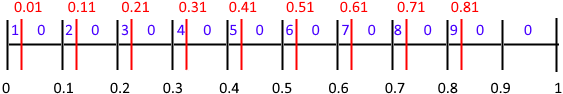
\includegraphics[width=\linewidth]{Walker.png}
\caption{Разбиение}
\label{fig:Walker}
\end{figure}
На рисунке черным обозначены границы базовых полуинтервалов, красным - границы полуинтервалов, синим - номера исходов, соответствующих данным полуинтервалам.